\chapter{Gestion des mails envoyés par le site web}
\label{gestion des mails}

\section{Modifier les mails}

Les différents mails générés par le site web sont placés dans un dossier \textit{mail} se trouvant dans le répertoire contenant les templates (voir figure~\ref{fig:Répertoire contenant les mails générés par le site web})

\begin{figure}[!ht]
    \centering
    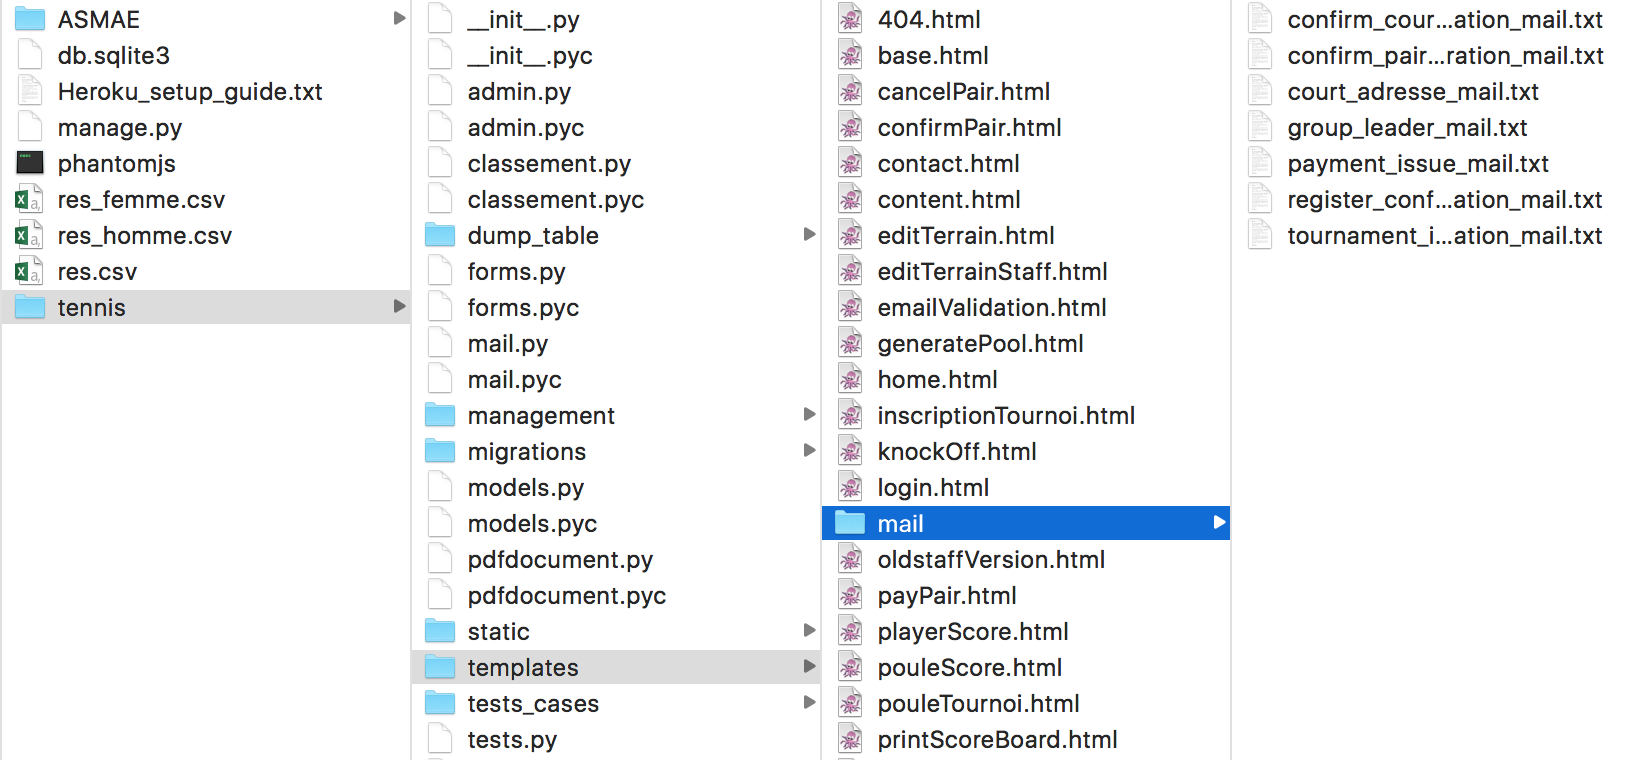
\includegraphics[width=0.7\linewidth]{developer_guide/mails.png}
    \caption{Répertoire contenant les mails générés par le site web}
    \label{fig:Répertoire contenant les mails générés par le site web}
\end{figure}
\FloatBarrier

Pour modifier les différents mails déjà existants, il suffit d'éditer le fichier texte correspondant au mail à modifier. Ces fichiers textes sont structurés de la même manière que celui présent sur la figure~\ref{fig:Exemple d'un fichier texte correspondant à un mail envoyé par le site web}. Le sujet du mail est contenu entre les balises \textit{<subject> ... </subject>} alors que le corps du mail est, quant à lui, entouré par les balises \textit{<message> ... </message>}.

\begin{figure}[!ht]
\begin{framed}
\begin{verbatim}
<subject>Le Charles de Lorraine : validation de votre adresse email<\subject>
<message>

Bonjour <<nameOne>>,

Afin de finaliser la création de votre compte 'Le Charles de Lorraine',  
merci de cliquer sur le lien suivant afin de validervotre adresse email.

<<link>>
	
Merci de votre cooperation,

L'équipe 'Le Charles de Lorraine'

<\message>
\end{verbatim}
\end{framed}
    \caption{Exemple d'un fichier texte correspondant à un mail envoyé par le site web}
    \label{fig:Exemple d'un fichier texte correspondant à un mail envoyé par le site web}
\end{figure}
\FloatBarrier

\section{Ajouter de nouveaux mails}

Pour permettre au site d'envoyer de nouveaux mails via certaines pages, il est d'abord nécessaire de créer un fichier texte comme présenté sur la figure~\ref{fig:Exemple d'un fichier texte correspondant à un mail envoyé par le site web} et de l'enregistrer dans le répertoire suivant: \textit{ASMAE/tennis/templates/mail}.

\todo[inline]{Expliquer comment le site peut envoyer les nouveaux mails}